\begin{enunciado}{\ejercicio}
  Factorizar en $\complejos[X]$ los polinomios
  \begin{enumerate}[label=\roman*)]
    \begin{multicols}{3}
      \item $X^2 + (1 + 2i)X + 2i$,
      \item $X^8 - 1$,
      \item $X^6 - (2 - 2i)^{12}$.
    \end{multicols}
  \end{enumerate}
\end{enunciado}

\begin{enumerate}[label=\roman*)]
  \item \textit{Si hay alguna raíz real} puedo igualar, la parte real e imaginaria a 0 para encontrarla:
        $$
          \blue{r}^2 + (1 + 2i)\blue{r} + 2i = 0
          \Sii{\red{!}}[$\blue{r} \en \reales$]
          \llave{rcl}{
            \blue{r}^2 + \blue{r} & = & 0 \\
            \ytext\\
            2i\blue{r} + 2i & = & 0
          }
          \Sii{raíz}[$\en \reales$]
          \blue{r} = -1
        $$
        Divido y queda listo:
        $$
          \divPol{X^2 + (1 + 2i)X + 2i}{X+1}
        $$
        Finalmente:
        $$
          \cajaResultado{
            X^2 + (1 + 2i)X + 2i = (X+1) \cdot (X +2i)
          }
        $$

  \item Raíces de la unidad \rollingEyes, lo mismo que se hizo siempre:
        $$
          X^8 - 1 = 0
          \sii
          X = e^{\frac{2\pi}{8}\cdot \blue{k}} ~ \text{con} ~ \blue{k} \en [0,7]
          \to
          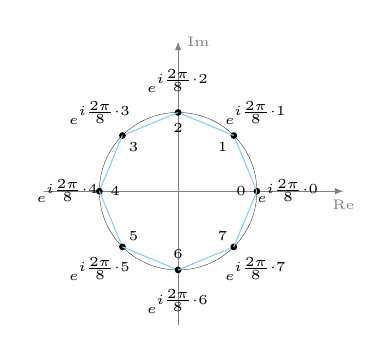
\begin{tikzpicture}[baseline=0, scale=1, every node/.style={font=\tiny}]
            \draw[ultra thin,-latex,gray] (-1.7,0) -- (2.1,0) node[below] {Re};
            \draw[ultra thin,-latex,gray] (0,-1.7) -- (0,1.9) node[right] {Im};
            \draw[ultra thin] (0,0) circle (1);
            \foreach \x in {0,...,8} {
                \ifnum \x < 8 {
                      \filldraw (\x*360/8:0.8) node {$\x$};
                      \filldraw (\x*360/8:1) circle (1pt);
                      \filldraw (\x*360/8:1.4) node {$e^{i \frac{2\pi}{8} \cdot \blue{\x}}$};
                      \draw[Cerulean!50] (\x*360/8:1) -- ({(\x+1)*360/8}:1);
                    }
                \fi
              }
          \end{tikzpicture}
        $$
        Pasando esas cosas a notación binómica queda la factorización:
        {\footnotesize
        $$
          \cajaResultado{
            \textstyle
            X^8 - 1 =
            (X - 1) \cdot
            (X + 1) \cdot
            (X - i) \cdot
            (X + i) \cdot
            (X - (\frac{1}{\sqrt{2}} + \frac{1}{\sqrt{2}})) \cdot
            (X - (\frac{1}{\sqrt{2}} - \frac{1}{\sqrt{2}})) \cdot
            (X - (-\frac{1}{\sqrt{2}} + \frac{1}{\sqrt{2}})) \cdot
            (X - (-\frac{1}{\sqrt{2}} - \frac{1}{\sqrt{2}}))
          }
        $$
        }

  \item Cuando tenemos exponentes grandes, se pasa a forma exponencial y ahí se labura. Hacer esto debería ser \textit{second nature} a esta
        altura, no obstante, acá va:
        $$
          \begin{array}{rcl}
            X^6 - (2 - 2i)^{12} = 0
                   & \sii                                &
            X^6  = (2 - 2i)^{12}                                                                                              \\
                   & \Sii{\red{!!}}[$X = r e^{i\theta}$] &
            r^6 \cdot e^{i 6\theta } = (2\sqrt{2})^{12} \cdot e^{i \frac{7}{4} \cdot 12 \pi}                                  \\
                   & \sii                                &
            r^6 \cdot e^{i 6\theta } = (2\sqrt{2})^{12} \cdot e^{i 21\pi} \igual{\red{!}} 8^6 \cdot e^{i\pi}                  \\
                   & \sii                                &
            \llave{rcl}{
            r      & =                                   & 8                                                                  \\
            \theta & =                                   & \frac{1}{6} \pi + \red{\frac{1}{3}k\pi} ~ \text{con} ~ k \en [0,5]
            }
          \end{array}
        $$
        Queda como $G_6$, pero con otro módulo, ponele:~ ~ ~
        $
          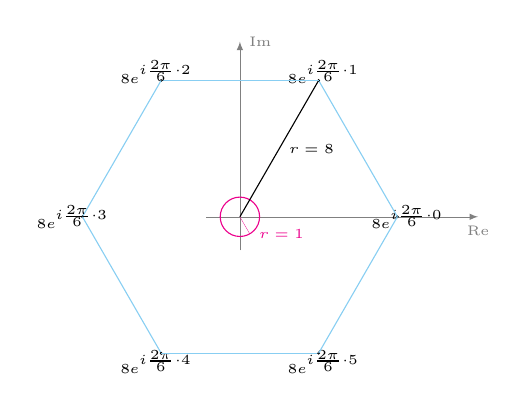
\begin{tikzpicture}[baseline=0, scale=0.25, every node/.style={font=\tiny}]
            \draw[ultra thin,-latex,gray] (-1.7,0) -- (12.1,0) node[below] {Re};
            \draw[ultra thin,-latex,gray] (0,-1.7) -- (0,8.9) node[right] {Im};
            \draw[thin, magenta] (0,0) circle (1); 
            \draw[thin] (0,0) -- (1*360/6:8) node[midway, right]{$r = 8$};
            \draw[ultra thin, magenta] (0,0) -- (5*360/6:1) node[right]{$r = 1$};
            \foreach \x in {0,...,6} {
                \ifnum \x < 6 {
                      \filldraw (\x*360/6:8) circle (1pt);
                      \filldraw (\x*360/6:8.5) node {$8e^{i \frac{2\pi}{6} \cdot \blue{\x}}$};
                      \draw[Cerulean!50] (\x*360/6:8) -- ({(\x+1)*360/6}:8);
                    }
                \fi
              }
          \end{tikzpicture}
        $

        Pasando esas cosas a forma binómica:
        {
        \small
        $$
          \textstyle
          \cajaResultado{
            X^6 - (2-2i)^{12} =
            \big(X - 8i\big)
            \big(X + 8i\big)
            \big(X - (4\sqrt{3} + 4i)\big)
            \big(X - (4\sqrt{3} - 4i)\big)
            \big(X - (-4\sqrt{3} + 4i)\big)
            \big(X - (-4\sqrt{3} - 4i)\big)
          }
        $$
        }
\end{enumerate}

\begin{aportes}[2]
  \item \aporte{https://github.com/ivdou}{Ivan Doumerc \github}
  \item \aporte{\dirRepo}{naD GarRaz \github}
\end{aportes}
